\setcounter{chapter}{0}

\boilerplatechapterone{%

The \ModelDesc\ provides a framework for representation of the gravity effects
of planetary bodies. The basic model is generic and extensible to allow
implementation of any common type of gravity field representation method. The
basic model also provides the simple point-mass gravitational attraction
calculations common to all Newtonian gravity representations to reduce
redundant effort when extending the model.

For increased computational efficiency, the basic gravity framework provided
allows the gravitational calculations to be controlled for each simulated
object independent of other objects. For example, the same planetary body
can be specified to have simple point-mass gravitational effects on one
object, while simultaneously being specified to provide high-order effects
on another. Gravitational attraction calculations can also be controlled per
planetary body for each simulated object, so that some planets can be acting
on an object as point-masses while others are simultaneously acting on the
same object with non-point-mass effects.

An extension of the basic model that uses a recursive, stable, and singularity--
free spherical harmonics algorithm to model gravity fields is also provided
as part of JEOD. This algorithm computes the gravitational acceleration acting
on an object due to the gravity of planetary bodies; it can also include the
effects of solid body tides in those calculations if desired. The model also
outputs the gradient of the gravitational acceleration, which can be used for
calculating gravitational torque or other microgravity effects.

A basic set of data files has been included along with the provided spherical
harmonics gravity implementation. These data files include the spherical
harmonic gravity coefficients for Earth, the Moon, and other planetary bodies
commonly included in simulations using JEOD. Model users can easily add
additional sets of gravity coefficients for these or any other planetary body
as required for their purposes.
} {%
   \ModelHistory
}


%----------------------------------
\chapter{Product Requirements}\hyperdef{part}{reqt}{}\label{ch:reqt}
%----------------------------------
This chapter describes the requirements for the \ModelDesc.

\requirement{Top-level}
\label{reqt:toplevel}
\begin{description}
\item[Requirement:]\ \newline
  This model shall meet the JEOD project requirements specified in the 
  \JEODid\ \hyperref{file:\JEODHOME/docs/JEOD.pdf}{part1}{reqt}{ top-level
  document}.
\item[Rationale:]\ \newline
  This model shall, at a minimum, meet all external and internal requirements
  applied to the \JEODid\ release.
\item[Verification:]\ \newline
  Inspection
\end{description}

\requirement{Extensibility}
\label{reqt:extensible}
\begin{description}
\item[Requirement:]\ \newline
  The \ModelDesc\ shall be extensible.
\item[Rationale:]\ \newline
  Extensibility allows custom, or multiple, methods of representing
  gravitational effects to be used in a simulation that employs the \ModelDesc.
\item[Verification:]\ \newline
  Inspection
\end{description}

\section{Data Requirements}\label{sec:data_reqts}
This section identifies requirements on the data 
represented by the \ModelDesc. These as-built requirements are based on
the \ModelDesc\ data definition header files.

\requirement{Generic Model Data}
\label{reqt:generic_data}
\begin{description}
  \item[Requirement:]\ \newline
The \ModelDesc\ shall provide a set of data fields denoting active status
and other generic settings to facilitate use of the model in simulations.
  \item[Rationale:]\ \newline
The primary function of the basic \ModelDesc\ framework is to provide
these generic settings and interfaces that apply to all gravity representation
methods.
  \item[Verification:]\ \newline
Inspection
\end{description}

\requirement{Spherical Harmonics Gravitational Data}
\label{reqt:spherharm_data}
\begin{description}
  \item[Requirement:]\ \newline
In the provided spherical harmonics gravity model extension, gravitational
potential shall be modeled by spherical harmonic expansion. The data for
the extension shall consist of unit-less gravity coefficients and
associated constants.
  \subrequirement{Gravity coefficients shall be fully 
normalized (cf. ~\cite{heiskanen1967,montenbruck2000,vallado2001}).}
  \subrequirement{All zero-order $S$ coefficients shall equal zero $(S_{n0}=0)$.}
  \subrequirement{Coefficient $C_{00}$ shall be exactly one $(C_{00}=1)$, and all 
first-degree coefficients shall be exactly zero $(C_{10}=C_{11}=S_{11}=0)$.} 
  \item[Rationale:]\ \newline
The functions in the provided spherical harmonics gravity model extension
utilize fully normalized gravity coefficients. The functions begin computing
with degree two $(n=2)$ coefficients.  The degree-zero and degree-one
coefficients are assumed to be the values listed above.
  \item[Verification:]\ \newline
Inspection
\end{description}

\section{Functional Requirements}\label{sec:func_reqts}
This section identifies requirements on the functional 
capabilities provided by the \ModelDesc.  These as-built requirements are
based on the \ModelDesc\ source files.

\requirement{Generic Model Functionality}
\label{reqt:generic_func}
\begin{description}
  \item[Requirement:]\ \newline
The \ModelDesc\ shall provide basic functionality required to enable all
extensions of the model to properly interface with JEOD.
  \subrequirement{The \ModelDesc\ shall provide a set of generic initialization
functions.}
  \subrequirement{The \ModelDesc\ shall provide a set of generic update
functions.}
  \subrequirement{The \ModelDesc\ shall provide simple point-mass gravitational
calculations.}
  \item[Rationale:]\ \newline
The primary function of the basic \ModelDesc\ framework is to provide
these generic functional interfaces that apply to all gravity representation
methods.
  \item[Verification:]\ \newline
Inspection for subrequirements 1 and 2, Test for subrequirement 3.
\end{description}

\requirement{Spherical Harmonics Gravitational Acceleration}
\label{reqt:spherharm_grav_accel}
\begin{description}
\item[Requirement:]\ \newline
The model shall compute the inertial acceleration vector due to a planetary
body at a specified position external to the body. The acceleration vector
shall be computed in the planet-fixed coordinate frame and transformed into
inertial coordinates. The model must be non-singular for polar orbits and
stable for high degree and order gravity fields.
\item[Rationale:]\ \newline
This describes the essential functionality of the spherical harmonics gravity
model extension. The acceleration due to gravity will be transformed into 
inertial coordinates for integration in the spacecraft equations of motion.
\item[Verification:]\ \newline
Test
\end{description}

\requirement{Spherical Harmonics Gravity Gradient}
\label{reqt:spherharm_grav_grad}
\begin{description}
\item[Requirement:]\ \newline
The model shall compute the gradient of the inertial gravity acceleration vector
due to a planetary body at a specified position external to the body. The model
shall provide the capability to specify the gravity gradient degree and order
independently from the acceleration degree and order.
\item[Rationale:]\ \newline
The gravity gradient is required for computing gravity torque and other
microgravity purposes.
\item[Verification:]\ \newline
Test
\end{description}

\requirement{Spherical Harmonics Solid Body Tides}
\label{reqt:spherharm_solid_tides}
\begin{description}
  \item[Requirement:]\ \newline
This model shall include the first-order effects of solid body tides acting on 
a planetary body due to any other planetary body (i.e., moon acting on
Earth, sun acting on moon, etc.)
  \item[Rationale:]\ \newline
Solid body tidal effects are required for high precision orbit modeling.
  \item[Verification:]\ \newline
    Test
\end{description}

%%% Format for the model Requirements is open.  It should include requirements for this model 
%%% only and use requirment tags like the one below.
%\requirement{...}
%\label{reqt:...}
%\begin{description}
%  \item[...]\ \newline
%    The documentation for the model shall include
%
%    \subrequirement{}
%    \label{reqt:...}
%      Software requirements specification.
%      
%    ...
%   
%  \item[title]\ \newline
%    text
%
%  ...
%
%\end{description}

%----------------------------------
\chapter{Product Specification}\hyperdef{part}{spec}{}\label{ch:spec}
%----------------------------------

\section{Conceptual Design}
\subsection{Basic Model}
The \ModelDesc\ provides a framework for representation of the gravity effects
of planetary bodies. The model is generic and extensible to allow
implementation of any common type of gravity field representation method. The
basic model also provides the simple point-mass gravitational attraction
calculations common to all Newtonian gravity representations to reduce
redundant effort when extending the model.

For increased computational efficiency, the basic gravity framework provided
allows the gravitational calculations to be controlled for each simulated
object independent of other objects. For example, the same planetary body
can be specified to have simple point-mass gravitational effects on one
object, while simultaneously being specified to provide high-order effects
on another. Gravitational attraction calculations can also be controlled per
planetary body for each simulated object, so that some planets can be acting
on an object as point-masses while others are simultaneously acting on the
same object with non-point-mass effects.

The generic gravity model can be easily extended to employ multiple types of
gravity representation methods simultaneously, not only running in the same
simulation but also acting upon the same object(s) at the same time. One such
extension of the generic model has been provided as part of the JEOD package
in the form of the spherical harmonics gravity implementation; this model
extension will be the primary focus of much of this chapter. 

\subsection{Spherical Harmonics Implementation}
The spherical harmonics gravity implementation is an extension of the basic
gravity model that uses a recursive, stable, and singularity-free spherical
harmonics algorithm to model gravity fields. This implementation can also
include the effects of solid body tides in those calculations if desired. The
model additionally outputs the gradient of the gravitational acceleration,
which can be used for calculating gravitational torque or other microgravity
effects.

The spherical harmonics implementation must be provided with a set of gravity
coefficients corresponding to a particular gravity field to perform its
calculations. These coefficients must be in fully normalized form. However, so
long as the given file is properly formatted and the coefficients are
normalized, any set of spherical harmonics gravity coefficients may be used
with the extended model; no code modification is required.

The gravitational acceleration and gradient calculations in this implementation
are adapted from the Ada code of Gottleib~\cite{JSC23762}. The solid body tide
model is the first-order model of the International
Earth Rotation and Reference Systems Service (IERS) ~\cite{IERS2003}.


%%%%%%%%%%%%%%%%%%%%%%%%%%%%%%%%%%%%%%%%%%%%%%%%%%%%%%%%%%%%%%%%%%%%%%%%%%%%%%%%
\section{Mathematical Formulations}

\subsection{Coordinate Systems}\label{sec:coordinates}
Gravitational fields are typically developed and expressed 
in spherical\footnote{Here the term
{\it spherical} means coordinates base on a spherical body as opposed to an
oblate elliptical body (i.e., geocentric vs. geodetic coordinates).},
planet-fixed coordinates. The symbols $(r,\lambda,\phi)$ are the spherical
coordinates radius, longitude, and latitude (Figure \ref{fig:sphere_cord}).
\begin{figure}[h]
\centering
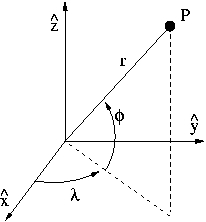
\includegraphics[width=2in]{figs/sphere.jpg}
\caption{Spherical coordinates.}
\label{fig:sphere_cord}
\end{figure}
The coordinate frames in which the fields are developed are typically
planet-fixed, that is, fixed with respect to the planetary body and,
therefore, are generally non-inertial.

Note: the spherical harmonics model extension is based on the
Gottlieb~\cite{JSC23762} formulation, which uses rectangular (i.e., Cartesian)
coordinates $(x,y,z)$.  The conversion from spherical to rectangular
coordinates is inherent in the extension's routines.

Typcially, the equations of motion of a spacecraft are expressed in 
inertial coordinates.  Therefore, a transformation is usually required
to express the gravitational acceleration and gradient in inertial coordinates.
This transformation is performed by the \ModelDesc\, but the required
transformation matrix is computed externally to the model.  In general,
the transformation matrix incorporates effects such as planetary rotation,
nutation, and precession; it is often referred to as the
{\it RNP matrix}\footnote{Other effects, such as polar motion, can be included
in the RNP matrix.}. For high precision work it is important to use the
planet-fixed coordinate system of the gravity field that is being used for each
gravitational body.

%%%%%%%%%%%%%%%%%%%%%%%%%%%%%%%%%%%%%%%%
\subsection{Spherical Harmonics Gravitational Potential}
A gravitational potential field model can be used to compute acceleration
(i.e., force per mass) acting on an object.  Most large planetary bodies
are predominately spherical in shape, but are not perfect spheres of uniform
mass distribution. The potential due to nonspherical bodies must be considered
for precision orbit modeling; spherical harmonics have been found to be a useful
way to model these non-ideal effects.

Gravitational potential can be expressed in spherical coordinates
as~\cite{montenbruck2000, vallado2001}
\begin{equation}
\label{eqn:basicU}
U(r,\lambda,\phi)=\frac{\mu}{r}\sum_{n=0}^\infty\sum_{m=0}^n
\left(\frac{R}{r}\right)^n\bar{P}_{n,m}(sin\phi)(\bar{C}_{n,m}\cos
m\lambda+\bar{S}_{n,m}\sin m\lambda)
\end{equation}
where $(r,\lambda,\phi)$ are the spherical coordinates radius, 
longitude, and latitude (Figure \ref{fig:sphere_cord}),
$\mu$ is the gravitational parameter 
$(\mu=GM)$; $n$ and $m$ are model degree and order; $R$ is the 
mean equatorial radius of the gravitational body; $\bar{P}_{n,m}$ is the fully 
normalized associated Legendre function of degree $n$ and order $m$;
and $\bar{C}_{nm}$ and 
$\bar{S}_{nm}$ are fully normalized unit-less gravity coefficients 
that are related to the mass distribution of the
body~\cite{kaula1966,montenbruck2000}. The overhead bar denotes a coefficient
that is fully normalized using the relationship
\begin{equation}\label{fullynormalize}
\left\{
\begin{array}{c}
\bar{C}_{nm}\\
\bar{S}_{nm}\\
\end{array}
\right\}=\sqrt{\frac{(n+m)!}{(2-\delta_{0m})(2n+1)(n-m)!}} \left\{
\begin{array}{c}
C_{nm}\\
S_{nm}\\
\end{array}
\right\}
\end{equation}
where $\delta_{0m}=1$ when $m=0$, and $\delta_{0m}=0$ when $m\neq0$.

The zero-degree term $(C_{00})$ represents the spherical surface 
upon which the higher degree terms are imposed. It is unity by definition
$(C_{00}=1)$.
All $\bar{S}_{nm}$ terms vanish for $m=0$ because the sine term in equation
\ref{eqn:basicU} vanishes when $m=0$
$(\sin 0=0)$.  It can be shown~\cite{montenbruck2000,torge2001} that the
location of the center of mass $(\bar{x},\bar{y},\bar{z})$ of the gravitational
body is related to the un-normalized first degree coefficients by
\begin{equation}\label{degree1coefficients}
\begin{aligned}
\bar{x} &=R C_{11}\\
\bar{y} &=R S_{11}\\
\bar{z} &=R C_{10}\\
\end{aligned}
\end{equation}
The normal practice is to define the spherical coordinate system such that the
origin is located at the center of mass. Therefore, the first degree terms
$C_{10}$, $C_{11}$, and $S_{11}$ all equal zero.  With these definitions of the
zero-degree and first-degree terms, the spherical harmonic model becomes
\begin{equation}
\label{spherharmon2}
U(r,\lambda,\phi)=\frac{\mu}{r}\left[1+\sum_{n=2}^\infty\sum_{m=0}^n
\left(\frac{R}{r}\right)^n\bar{P}_{n,m}(sin\phi)(\bar{C}_{n,m}\cos
m\lambda+\bar{S}_{n,m}\sin m\lambda)\right]
\end{equation}
For a large continuous body of mass (i.e., a planet) the gravity coefficients
are related to the mass distribution by
\begin{equation}\label{CandSdefined}
\begin{aligned}
C_{nm}&=\frac{2-\delta_{0m}}{M}\frac{(n-m)!}{(n+m)!}\int\left(\frac{s}{R}\right)^n
P_{nm}\sin(\phi')\cos(m\lambda')\rho(s)d^3s\\
S_{nm}&=\frac{2-\delta_{0m}}{M}\frac{(n-m)!}{(n+m)!}\int\left(\frac{s}{R}\right)^n
P_{nm}\sin(\phi')\sin(m\lambda')\rho(s)d^3s\\
\end{aligned}
\end{equation}
where $(s,\lambda',\phi')$ are the spherical coordinates of each infinitesimal
particle of mass, $\rho(s)$ is density as a function of position within the
body of mass, and $d^3s$ indicates volume integration over the entire body of
mass~\cite{montenbruck2000}.

%%%%%%%%%%%%%%%%%%%%%%%%%%%%%%%%%%%%%%%%
\subsection{Gravitational Acceleration}
The acceleration in rectangular coordinates due to gravity is found by computing
the gradient of the gravitational potential.
\begin{equation}
\bar{a} =  \nabla U
\end{equation}
To satisfy the functional requirement that the spherical harmonics extension of
the \ModelDesc\ be non-singular and stable, acceleration is efficiently computed
in rectangular coordinates using recursion equations for the Legendre polynomials.
The technique used is that of Gottlieb as detailed in
\hyperref{file:\JEODHOME/models/environment/gravity/docs/gottlieb_1993.pdf}{part1}{reqt}
{Fast Gravity, Gravity Partials, Normalized Gravity, Gravity Gradient 
Torque, and Magnetic Field: Derivation, Code, and Data}~\cite{JSC23762}.  

Simple point-mass gravitational acceleration is calculated by the base
\ModelDesc\ using the standard two-body equation for gravitational attraction.

%%%%%%%%%%%%%%%%%%%%%%%%%%%%%%%%%%%%%%%%
\subsection{Gravity Gradient}
The gravity gradient is a 3x3 Jacobian (matrix) that is the partial derivative
of the inertial gravitational acceleration vector with respect to the inertial
position vector (rectangular coordinates).
\begin{equation}
\nabla \bar{a} = \frac{\partial\bar{a}}{\partial\bar{r}} =
\left[
\begin{array}{ccc}
\partial{a_x}/\partial{x} & \partial{a_x}/\partial{y} & \partial{a_x}/\partial{z} \\
\partial{a_y}/\partial{x} & \partial{a_y}/\partial{y} & \partial{a_y}/\partial{z} \\
\partial{a_z}/\partial{x} & \partial{a_z}/\partial{y} & \partial{a_z}/\partial{z} \\
\end{array}
\right]
\end{equation}

The spherical harmonics extension of the \ModelDesc\ uses Gottlieb's method for
computing gravity gradient~\cite{JSC23762}. Gottlieb's method computes the
gradient due to the full gravity field. It does not make any simplifying
assumptions such as a spherical or simple oblate gravitational body.

The base \ModelDesc\ computes spherical gravity gradient using the analytic
solutions for the partial derivatives of the simple point-mass acceleration.

The trace of the gravity gradient matrix (sum of the diagonal terms) is the
Laplacian of the gravitational potential and is equal to zero for any
gravity field.
\begin{equation}
\nabla^2 U = \frac{\partial^2U}{\partial x^2}+\frac{\partial^2U}{\partial y^2}+\frac{\partial^2U}{\partial z^2} =
\frac{\partial a_x}{\partial x}+\frac{\partial a_y}{\partial y}+\frac{\partial a_z}{\partial z} = 0
\end{equation}
where $U$ is the gravitational potential (equation \ref{spherharmon2}).

The gravity gradient can be used to compute gravity torque. Consult the JEOD
\hyperref{file:\JEODHOME/models/interactions/gravity_torque/docs/gravity_torque.pdf}{part1}{reqt}
{Gravity Torque Model} document for detail~\cite{dynenv:gravitytorque}. Gravity
gradient can also be used for microgravity and other similar purposes.


%%%%%%%%%%%%%%%%%%%%%%%%%%%%%%%%%%%%%%%%
\subsection{Solid Body Tides}
In general, the large planetary bodies of the solar system are not perfectly
rigid. They deform in response to the gravitational forces of other large
bodies acting upon them, resulting in temporal variations of mass
distribution known as {\it tides}. Deformation results in a change in the mass
distribution of the planetary body which, in turn, causes a change in its
spherical harmonics gravity coefficients (equations \ref{CandSdefined}).
The term {\it solid body tide} refers to the large-scale tidal response of
the entire planetary body, which is different from the tidal response of
oceans and atmospheres.

The solid body tide calculations in the spherical harmonics extension of the
\ModelDesc\ is the first-order model of the International Earth Rotation and
Reference System Service (IERS) Conventions 2003~\cite{IERS2003}; note that
solid body tides are not calculated by the base \ModelDesc\, since it models
planetary bodies as simple point-masses that are not capable of deformation.
The model is expressed as a change in the normalized gravity coefficients as
%\begin{equation}
%\Delta \bar{C}_{2,0} = \frac{k_2}{5}\sum_{j=2}^3\frac{\mu_j}{\mu_E}
%\left(\frac{R_E}{r_j}\right)^3\sqrt{5}\left(\frac{3}{2}\sin^2\phi-\frac{1}{2}\right)
%\end{equation}
\begin{equation}
\Delta\bar{C}_{nm}-i\Delta\bar{S}_{nm} = \frac{k_{nm}}{2n+1}\sum_{j}
\frac{\mu_j}{\mu}\left(\frac{R}{r_j}\right)^{n+1}\bar{P}_{nm}\left(\sin\phi_j\right)e^{-im\lambda_j}
\end{equation}
where 
\begin{description}
\item{$k_{nm}$ is the elastic Love number of the central body}
\item{$j$ is the index of each tidal producing body}
\item{$\mu_j$ is the gravitational parameter of the tidal producing body}
\item{$\mu$ is the gravitational parameter of the central body}
\item{$R$ is the equatorial radius of the central body}
\item{$r_j$ is the distance to the tidal producing body (assume point mass)}
\item{$\phi_j$ is the spherical latitude of the tidal producing body}
\item{$\lambda_j$ is the spherical longitude of the tidal producing body}
\end{description}

Euler's formula $(e^{ix}=\cos x +i\sin x)$ can be used to write separate
equations for the gravity coefficient changes.
\begin{equation}
\Delta\bar{C}_{nm}= \frac{k_{nm}}{2n+1}\sum_{j=2}^n
\frac{\mu_j}{\mu}\left(\frac{R}{r_j}\right)^{n+1}\bar{P}_{nm}\left(\sin\phi_j\right)\cos m\lambda_j
\end{equation}
\begin{equation}
\Delta\bar{S}_{nm}= \frac{k_{nm}}{2n+1}\sum_{j=2}^n
\frac{\mu_j}{\mu}\left(\frac{R}{r_j}\right)^{n+1}\bar{P}_{nm}\left(\sin\phi_j\right)\sin m\lambda_j
\end{equation}

In general, the tidal effect on the $\bar{C}_{20}$ gravity coefficient does not
average to zero over time.  The non-zero mean effect is called the
{\it permanent tide} or the {\it zero frequency tide}.  The effect can be
included in the {\it a priori} gravity field model.  If it is, care must be
taken to remove this effect when modeling solid body tides.  Otherwise, the
permanent tide effect will be erroneously included twice in the tide model.
Whether or not the permanent tide is included in a particular gravity field is
usually specified in supporting documentation.  For Earth, the permanent tide
effect can be removed using~\cite{IERS2003,Seidelmann}
\begin{equation}
\Delta\bar{C}_{20}= -4.4228\times10^{-8}(-0.31460)k_{20}
\end{equation}


%%%%%%%%%%%%%%%%%%%%%%%%%%%%%%%%%%%%%%%%%%%%%%%%%%%%%%%%%%%%%%%%%%%%%%%%%%%%%%%
\section{Detailed Design}

The general algorithm used by the spherical harmonics extension of the
\ModelDesc\ is that of Gottlieb as detailed in
\hyperref{file:\JEODHOME/models/environment/gravity/docs/gottlieb_1993.pdf}{part1}{reqt}
{Fast Gravity, Gravity Partials, Normalized Gravity, Gravity Gradient Torque,
and Magnetic Field: Derivation, Code, and Data}~\cite{JSC23762}.  Each simulated
spacecraft has gravity controls that select the size (degree and order) of the
gravity field for each planetary body acting on the spacecraft.  Each
spacecraft also controls the gradient and tide effects of each body.  The degree
and order controls for the gravity gradient can be set independently from the
degree and order of the gravity acceleration controls\footnote{This required a
functional modification to Gottlieb's original algorithm.}.  However, the
gradient degree and order must be less than or equal to the acceleration degree
and order.  If the gradient controls are not specified by the user, the
\ModelDesc\ will default to the gradient of a spherical body as calculated by
the base model regardless of the gravity control settings for acceleration.


%%%%%%%%%%%%%%%%%%%%%%%%%%%%%%%%%%%%%%%%
\subsection{Third Body Gravity} \label{sssec:ThirdBody}

Third body gravity describes the gravitational acceleration of a vehicle $V$
toward a third body $B$, as expressed in a frame $F$ whose origin is also
accelerating gravitationally toward the same third body.
Let $\vect \rho$, $\vect r$ and $\vect d$ be the vectors from the origin
of the accelerating frame to $B$, from the origin to $V$, and from $B$ to $V$.
(Note that $\vect d = \vect r - \vect \rho$.)

The gravitational acceleration of the vehicle in an inertial frame $I$ toward
the body with gravitational parameter $\mu$ is
\begin{align}
\vect a_{V\to B,I} &= - \mu \frac {\vect d}{d^3} \\
\intertext{The origin of the frame is also accelerating gravitationally toward
$B$:}
\vect a_{O\to B,I} &= \phantom{-} \mu \frac {\vect \rho}{\rho^3} \\
\intertext{The difference between the above two vectors yields the acceleration
of the vehicle toward the body in the accelerating frame:}
\vect a_{V\to B,F}
  &= - \mu \left( \frac {\vect d} {d^3} + \frac {\vect \rho} {\rho^3} \right)
  \label{addedform}
\end{align}

Equation \eqref{addedform} can suffer from precision loss when $r \ll \rho$
as the vectors $\frac{\vect d}{d^3}$ and $\frac{\vect \rho}{\rho^3}$
are close to additive inverses of one another in this case. 

\subsubsection{Development of a Robust Expression}
The goal is to develop an equivalent expression that avoids precision loss.
The development follows that of Battin in
\emph{Introduction to the Mathematics and Methods of Astrodynamics}.
Factoring out $1/d^3$ from equation \eqref{addedform}
and using $\vect d = \vect r - \vect \rho$ yields
\begin{align}
\vect a_{V\to B,F}
  &= -\,\frac {\mu}{d^3}
     \left(  \vect r
           + \vect \rho \left(\frac {d^3}{\rho^3} - 1\right) \right)
  \label{scalarform}
\end{align}

The above remains problematic because $\frac {d^3}{\rho^3}$ will be very
close to one in the case $r \ll \rho$.
The solution is to express $f \equiv \frac {d^3}{\rho^3} - 1$ in a manner that
does not involve the subtraction.
Multiplying $f$ by one, where one is written as
$\frac{\frac {d^3}{\rho^3} + 1}{\frac {d^3}{\rho^3} + 1}$
results in
\begin{align}
f &= \frac {d^3}{\rho^3} - 1 \nonumber \\
  &= \frac {\left(\frac {d^3}{\rho^3} - 1\right)
            \left(\frac {d^3}{\rho^3} + 1\right)} 
           {\frac {d^3}{\rho^3} + 1} \nonumber \\
  &= \frac {\left(\frac {d^2}{\rho^2}\right)^3 - 1}
           {\left(\frac {d^2}{\rho^2}\right)^{3/2} + 1}
\label{multipled_by_one} \\
\intertext{To simplify the calculation, denote $q$ and $\delta$ by}
q &\equiv \frac {d^2}{\rho^2} - 1 \nonumber \\
&= \frac{\rho^2 - 2\,\vect r \cdot \vect \rho + r^2}{\rho^2} - 1 \nonumber \\
& = \frac{\vect r \cdot (\vect r - 2 \vect \rho)}{\rho^2} \label{q} \\
\delta &\equiv (q+1)^3 - 1 \nonumber \\
&= q(3+q(3+q)) \label{delta} \\
\intertext{With this, equation \eqref{multipled_by_one} becomes}
f &=
\frac {(q+1)^3 - 1}{(q+1)^{3/2} + 1} \nonumber \\
&= \frac{\delta}{1+\sqrt{1+\delta}} \label{f} \\
\intertext{Finally, equation \eqref{scalarform} becomes}
\vect a_{V\to B,F}
  &= -\,\frac {\mu}{\rho^3} \frac{\vect r + f \vect \rho}{1+f}
\label{finalform}
\end{align}

Note that the above avoids precision loss because of how $q$, $\delta$,
and $f$ are calculated in equations \eqref{q} to \eqref{f}.
Note also that equation \eqref{finalform} avoids having to calculate the
vector $\vect d$.

\subsection{Reference Manual}

The complete API for the \ModelDesc\ can be found in the
\href{file:refman.pdf}{\em Reference Manaual} ~\cite{gravity_refman}.

\clearpage
\boilerplateinventory


%----------------------------------
\chapter{User Guide}\hyperdef{part}{user}{}\label{ch:user}
%----------------------------------
The User Guide is divided into three instruction sets:
\begin{enumerate}
 \item \textbf{Instructions for Simulation Users}.  This instruction-set
 contains a description of how to modify \ModelDesc\ variables after the
 simulation has compiled, including a discussion of the input file;
 an overview of how to interpret (but not edit) the S\_define file; and a
 sample of some of the typical variables that may be logged.
 \item \textbf{Instructions for Simulation Developers}.  This instruction-set
 builds on the previous set, and adds information on the necessary
 configuration of the \ModelDesc\ within an S\_define file, and the creation of
 standard run directories.
 \item \textbf{Instructions for Model Developers}.   This instruction-set
 builds on the previous set, and adds information on the potential for
 extending the model to perform tasks that are beyond its current abilities.
\end{enumerate}

Note that the \ModelDesc\ has been reworked to allow for
other types of gravity representations than spherical harmonics, the
default for \JEODid\ remains the spherical harmonics extension of the model.
Thus, this implementation is the primary one discussed in this chapter, though
the Model Developers section briefly discusses how to implement an alternative
gravity representation.

%%%%%%%%%%%%%%%%%%%%%%%%%%%%%%%%%%%%%%%%%%%%%%%%%%%%%%%%%%%%%%%%%%%%%%%%%%%%%%%%
\section{Instructions for Simulation Users}

\subsection{Spherical Harmonics Gravity Fields}
The gravity field to be used for each gravitational body is specified in the
Trick sim object for each body in the S\_define file. The specified spherical
harmonics coefficients are loaded into the \ModelDesc\ at sim initialization
(i.e., each time the sim is run). The gravity fields provided with the current
version of JEOD are found in the {\bf environment/gravity/data} directory. Other
gravity fields can be easily added to this directory by JEOD users\footnote{As
explained in section \ref{sec:coordinates}, each gravity field is developed in
a specific planet-fixed coordinate system. To support high precision analysis,
new gravity fields should be introduced with their corresponding planet-fixed
frames.}. Care must be taken to ensure the gravity coefficients are in the
correct format.  Whether using the existing data files or adding new ones, users
should note that for all spherical harmonics gravity fields, the first three
terms of SphericalHarmonicsGravitySource.Cnm are always the same and have thus
been hard-coded into the model. So, any value entered for them in the data file
is ignored by the gravity routines.  The same holds true for the first three
terms of SphericalHarmonicsGravitySource.Snm.

Example code is given for Trick users; non-Trick users should follow a similar
pattern using their appropriate syntax.  An example from an S\_define sim
object that selects the GGM02C gravity field for Earth is:

\begin{verbatim}
 ##include "environment/gravity/include/spherical_harmonics_gravity_source.hh"
 ##include "environment/gravity/data/include/earth_GGM02C.hh"

   SphericalHarmonicsGravitySource   gravity_source;
   SphericalHarmonicsGravitySource_earth_GGM02C_default_data
                                   gravity_source_default_data;
   ("default_data") gravity_source_default_data.initialize ( &gravity_source );
\end{verbatim}


\subsection{Gravity Controls}
The effects of gravity for each gravitational body in each sim are controlled
on a per-spacecraft basis.  Each spacecraft object has gravity controls that
determine whether the gravity field is spherical or nonspherical, the size
(degree/order) of a nonspherical field, whether the gravity gradient is
computed, and whether the full nonspherical field is computed or just the
perturbing component of the field.  Each of these controls is available for each
spacecraft and for each active gravitational body. The controls are intended
to be set by the user via the simulation input file.

An example declaration of the gravity controls in an S\_define file that
includes Earth, the sun, and the moon would be:
\begin{verbatim}
 ##include "environment/gravity/include/spherical_harmonics_gravity_controls.hh"

   SphericalHarmonicsGravityControls earth_grav_ctrl;
   SphericalHarmonicsGravityControls sun_grav_ctrl;
   SphericalHarmonicsGravityControls moon_grav_ctrl;
\end{verbatim}

Assuming these example gravity controls are declared in a Trick sim object
named sv\_dyn, a sample gravity controls setup for Earth in an input file
would then be:
\begin{verbatim}
   sv_dyn.earth_grav_ctrl.source_name     = "Earth";
   sv_dyn.earth_grav_ctrl.active          = True;
   sv_dyn.earth_grav_ctrl.spherical       = False;
   sv_dyn.earth_grav_ctrl.degree          = 70;
   sv_dyn.earth_grav_ctrl.order           = 70;
   sv_dyn.earth_grav_ctrl.gradient        = True;
   sv_dyn.earth_grav_ctrl.gradient_degree = 5;
   sv_dyn.earth_grav_ctrl.gradient_order  = 5;
   sv_dyn.earth_grav_ctrl.perturbing_only = False;
   sv_dyn.earth_grav_ctrl.battin_method   = False;
\end{verbatim}

If a spherical gravity field has been selected for a particular body, then
degree and order are ignored. If degree and order are not specified when
nonspherical gravity is selected, then the entire gravity field (maximum
degree and order available) is used by default.  This could cause a sim to run
much slower than it would otherwise run.  

The gradient control must be ``True'' in order to invoke the JEOD Gravity Torque
Model. The gradient degree and order must be less than or equal to the
acceleration degree and order. In this example, the gradient degree and order
are both 5, and the acceleration degree and order are both 70. If the gradient
degree and order are not specified, the \ModelDesc\ will compute the
spherical body gradient by default. Spherical body gradient can also be invoked
by setting the gradient degree and order both to 0. See  
\hyperref{file:\JEODHOME/models/interactions/gravity_torque/docs/gravity_torque.pdf}{part1}{reqt}
{JEOD Gravity Torque Model} ~\cite{dynenv:gravitytorque} for more information on
gravity torque.

The perturbing\_only control will default to false if not otherwise specified.
This will be the correct option for most sims running JEOD (i.e., spacecraft
trajectory simulations). This option was included because certain gravity field
analysis or advanced integration methods may require only the perturbing 
portion of the gravity field to be computed.

The battin\_method control determines whether an alternative formulation
of third body gravity will be used. The alternate method provides better
numerical accuracy at a slight cost in complexity. For a detailed description,
see ~\ref{sssec:ThirdBody}. The default value is false.

\subsection{Solid Body Tides}
Solid body tide effects are modeled as temporal variations in the gravity
coefficients of a gravitation body due to the gravity of one or more other
gravitational bodies (such as the sun or moon).  The tidal causing bodies are
selected via a default data file in the simulation S\_define.  After the solid
body tides have been properly included in the S\_define (see the next section
for how this is done), the sim user can ``turn off'' or ``turn on''
solid body tides from the input file by setting the ``active'' control to
``True'' or ``False.''

An example declaration of a solid body tide control in an S\_define file is:
\begin{verbatim}
 ##include "environment/gravity/include/spherical_harmonics_delta_controls.hh"
   SphericalHarmonicsDeltaControls sbtide_ctrl;
\end{verbatim}

Again assuming that this control was declared in a Trick sim object named
sv\_dyn, an example solid body tide control setup in the input file would be:
\begin{verbatim}
   earth.sb_tide.dC20 = 0.0;
   sv_dyn.sbtide_ctrl.active = True;
   sv_dyn.sbtide_ctrl.first_order_only = True;
   sv_dyn.sbtide_ctrl.degree = 2;
   sv_dyn.sbtide_ctrl.order = 0;
   sv_dyn.sbtide_ctrl.grav_effect = earth.sb_tide;
   sv_dyn.sbtide_ctrl.grav_source   = earth.gravity_source;
\end{verbatim}


\subsection{Data Logging}
An example line from a log file for recording gravitational acceleration
of a spacecraft is:
\begin{verbatim}
   for ii in range(0,3):
    dr_group.add_variable(""+VEH_OBJ+".body.grav_interaction.grav_accel["+str(ii)+"]")
\end{verbatim}


%%%%%%%%%%%%%%%%%%%%%%%%%%%%%%%%%%%%%%%%%%%%%%%%%%%%%%%%%%%%%%%%%%%%%%%%%%%%%%%%
\section{Instructions for Simulation Developers}

\subsection{Gravity Model}
The top-level structure for the \ModelDesc\ is normally declared as part of a
space environment sim object in the S\_define file for a simulation, such as:
\begin{verbatim}
 ##include "environment/gravity/include/gravity_manager.hh"
   GravityManager gravity;
\end{verbatim}

An initialization job is also required as part of the same sim object: 
\begin{verbatim}
   P_ENV  ("initialization") gravity.initialize_model (
      internal_dynamics->manager );
\end{verbatim}

Each planetary body must declare a gravity body object (note that the spherical
harmonics coefficients are normally loaded into this object as default data) and
call two initialization-related jobs. An example that uses the GRACE GGM02C
gravity field for Earth is:
\begin{verbatim}
 ##include "environment/gravity/include/spherical_harmonics_gravity_source.hh"
 ##include "environment/gravity/data/include/earth_GGM02C.hh"

   SphericalHarmonicsGravitySource   gravity_source;
   SphericalHarmonicsGravitySource_earth_GGM02C_default_data
                                   gravity_source_default_data;
   ("default_data") gravity_source_default_data.initialize ( &gravity_source );

   P_ENV  ("initialization") gravity_source.initialize_body ( );
   P_ENV  ("initialization") internal_env->gravity.add_grav_source(
      gravity_source );
\end{verbatim}

Each spacecraft object in the simulation will have its own set of gravity
controls that specify how these gravity bodies affect it. Implementation of
these controls requires declaration of the controls themselves. In the
S\_define, the set of controls are implemented as follows:
\begin{verbatim}
 ##include "environment/gravity/include/spherical_harmonics_gravity_controls.hh"

   SphericalHarmonicsGravityControls earth_grav_ctrl;
   SphericalHarmonicsGravityControls sun_grav_ctrl;
   SphericalHarmonicsGravityControls moon_grav_ctrl;
\end{verbatim}

The following corresponding lines would then go in the input file:
\begin{verbatim}
   sv_dyn.body.grav_interaction.add_control(sv_dyn.earth_grav_ctrl)
   sv_dyn.body.grav_interaction.add_control(sv_dyn.sun_grav_ctrl)
   sv_dyn.body.grav_interaction.add_control(sv_dyn.moon_grav_ctrl)
\end{verbatim}

The use of the settings within these controls was discussed in the previous
section and will not be repeated here.

\subsection{Gravity Interaction}
The gravity effects acting on an individual spacecraft are captured in a
gravity interaction class to which gravity controls are added as shown
above. The gravity interaction class offers a method to sort its gravity
controls so that their summation is performed in order of increasing magnitude.
This is a recommended practice for multi-planet simulations since the
additional overhead is minuscule, and it can significantly improve accuracy.
To sort at ten minute intervals, add the following line to your Trick 10
vehicle sim object.
\begin{verbatim}
(600, "environment") body.grav_interaction.sort_controls ();
\end{verbatim}

\subsection{Solid Body Tides}
To include solid body tides in a simulation, an object of type
SphericalHarmonicsSolidBodyTides must be included as part of the S\_define in
the relevant planet-related sim object; its companion initialization object
SphericalHarmonicsSolidBodyTidesInit must also be included.  For example, as
part of the Earth-related sim object, one could include:
\begin{verbatim}
 ##include "environment/gravity/include/spherical_harmonics_solid_body_tides.hh"
 ##include "environment/gravity/include/spherical_harmonics_solid_body_tides_init.hh"
 ##include "environment/gravity/data/include/earth_solid_tides.hh"

   SphericalHarmonicsSolidBodyTides       sb_tide;
   SphericalHarmonicsSolidBodyTidesInit   sbtide_init;
   SphericalHarmonicsSolidBodyTidesInit_earth_solid_tides_default_data
                                          sbtide_init_default_data;
   ("default_data") sbtide_init_default_data.initialize ( &sbtide_init );
\end{verbatim}

More information about these two objects can be found in
\hyperref{file:refman.pdf}{}{}
{JEOD Gravity Model Reference Manual} ~\cite{gravity_refman}. A call to job
``add\_deltacoeff'' must accompany these items (in the same sim object) for
proper functioning of the solid body tides:
\begin{verbatim}
   P31  ("initialization") gravity_source.add_deltacoeff (
      sbtide_init,
      internal_dynamics->manager,
      sb_tide );
\end{verbatim}

Each spacecraft object in the simulation will have its own set of controls that
specify how the solid body tides affect it. Similar to the controls for each
gravity body, implementation of the solid body tides controls requires
declaration of the controls themselves in the S\_define:
\begin{verbatim}
 ##include "environment/gravity/include/spherical_harmonics_delta_controls.hh"
   environment/gravity: SphericalHarmonicsDeltaControls sbtide_ctrl;
\end{verbatim}

The relevant input file entry that corresponds would then be:
\begin{verbatim}
   sv_dyn.earth_grav_ctrl.add_deltacontrol(sv_dyn.sbtide_ctrl)
\end{verbatim}

Once these elements are included, the \ModelDesc\ will automatically
incorporate the solid body tide calculations as appropriate based on the
relevant control settings.  Control of the solid body tides model was described
in the previous section.

%%%%%%%%%%%%%%%%%%%%%%%%%%%%%%%%%%%%%%%%%%%%%%%%%%%%%%%%%%%%%%%%%%%%%%%%%%%%%%%%
\section{Instructions for Model Developers}
There are two ways to extend the \ModelDesc: by incorporating additional
spherical harmonics gravity fields other than those provided as default data in
the {\bf environment/gravity/data} directory, and by implementing different
gravity representations other than spherical harmonics.

If incorporating a new spherical harmonics gravity field, care must be taken to
ensure the gravity coefficients are in the correct format.  All of the
coefficients must be in fully normalized form (see Chapter \ref{ch:spec}).

If implementing a new gravity representation, one must have familiarity with
the C++ programming language. The existing spherical harmonics extension of
the \ModelDesc\ might also prove to be a helpful guide for the implementation
process.

For the new model extension, two derived classes should be created: one that
inherits from GravitySource, and one that inherits from GravityControls. The
derived GravitySource-based class should contain any gravity representation--
related data; for example, the analogous class for the spherical harmonics
extension contains all of the Gottlieb parameters and spherical harmonics
coefficients necessary to perform the model's gravitational calculations.
The GravitySource-based class should also be primarily a container class, since
all gravitational calculations are performed in the GravityControls-based class.

The base GravityControls class has four methods: ``initialize\_control'',
``reset\_control'', ``gravitation'', and protected method
``calc\_nonspherical''. As their names imply, the first two methods contain
basic class initialization and reset functionality that will be common to all
gravity model representations. The model developer can optionally extend
either, both, or neither method as best suits his needs without affecting
overall \ModelDesc\ integrity, so long as any extensions still call the
base-class method(s). For reference, the spherical harmonics
implementation extends initialize\_control (while still invoking the base
method), but it leaves reset\_control untouched.

The base-class ``gravitation'' method converts the given position vector
into the proper frame and then performs the universal two-body point-mass
gravity calculation. This method is not intended to be overridden.

Base-class method ``calc\_nonspherical'' is the one method that \emph{must}
be overridden for successful model extension. The base method exists only for
inheritance and will throw an error if invoked. The overriding method
should contain any nonspherical gravity calculations for the new model
extension. If properly implemented, the derived-class method will
automatically be called by the \ModelDesc\ when an instance of the new
model extension is employed.


%----------------------------------
\chapter{Inspections, Tests, and Metrics}\hyperdef{part}{ivv}{}\label{ch:ivv}
%----------------------------------

\section{Inspections}
This section describes the inspections conducted on the \ModelDesc\ to
examine its compliance with the inspection requirements levied against it.

\inspection{Top-level Inspection}\label{inspect:TLI}
This document structure, the code, and associated files have been inspected,
and together satisfy requirement \traceref{reqt:toplevel}.

\inspection{Extensibility Inspection}\label{inspect:extensible}
The successful spherical harmonics extension of the model demonstrates
satisfaction of requirement \traceref{reqt:extensible}.

\inspection{Generic Model Data Inspection}\label{inspect:generic_data}
The model code has been inspected and satisfies requirement
\traceref{reqt:generic_data}.

\inspection{Spherical Harmonics Data Inspection}\label{inspect:spherharm_data}
The spherical harmonics code has been inspected and it satisfies requirement
\traceref{reqt:spherharm_data}.

\inspection{Generic Model Functionality Inspection}\label{inspect:generic_func}
The model code has been inspected, and it partially satisfies requirement
\traceref{reqt:generic_func}.

\section{Tests}
This section describes the verification and validation tests conducted on
the \ModelDesc\ to examine its satisfaction of the test requirements levied
against it. The tests described in this section are archived in the JEOD
directory \verb+models/environment/gravity/verif+. 

\test{Spherical Harmonics Gravity Acceleration Computation}
\label{test:spherharm_grav_accel}
\begin{description}
\item[Purpose:] \ \newline
The purpose of this test is to examine the spherical harmonics gravitational
accleration calculations against an analytic solution.\\
SIM directory: models/environment/gravity/verif/SIM\_grav\_accel\_verif\\
Run directory: RUN\_01
\item[Applicable Requirements:] \ \newline
By passing this test, the \ModelDesc\ satisfies requirement
\traceref{reqt:spherharm_grav_accel}.
\item[Procedure:]\ \newline
The gravity coefficients of a system of $i$ discrete point masses $(m_i)$ can be
obtained by reformulating equations \ref{CandSdefined} as
(see Thompson~\cite{thompson2008})
\begin{equation}\label{CandSdefinedptmasses}
\begin{aligned}
C_{nm}&=\frac{2-\delta_{0m}}{M_\oplus}\frac{(n-m)!}{(n+m)!}\sum_i\left(\frac{s_i}{R_\oplus}\right)^n
P_{nm}\sin(\phi'_i)\cos(m\lambda'_i)m_i\\
S_{nm}&=\frac{2-\delta_{0m}}{M_\oplus}\frac{(n-m)!}{(n+m)!}\sum_i\left(\frac{s_i}{R_\oplus}\right)^n
P_{nm}\sin(\phi'_i)\sin(m\lambda'_i)m_i\\
\end{aligned}
\end{equation}
The coefficients can be normalized using equation \ref{fullynormalize}. They can
be read into a gravity model, and the resulting acceleration can be compared
with the acceleration resulting directly from the point masses in order to
verify the spherical harmonic algorithms are working properly.

{\bf Point Mass System}

Because the goal of this work was to test the implementation of spherical
harmonic acceleration algorithms, the gravity coefficients used did not need to
truly represent any particular planet.  However, for familiarity it was decided
to choose a system of point masses that would produce accelerations on the same
scale that would be encountered by a low-Earth-orbiting satellite. For the
chosen point mass system, the constants of the JGM-3 (or GGM02C) gravity field
were used~\cite{MG}:
\begin{equation}\label{constants}
\begin{aligned}
\mu &= 398600.4415    \mbox{   $km^3/s^2$}\\
R_\oplus &= 6378.1363 \mbox{   $km$}
\end{aligned}
\end{equation}
Knowing that $\mu=GM_\oplus$ and assuming a value for $G$ of 
$6.673\times10^{-20}$ $km^3/(kg\cdot s^2)$, the total mass of the system of
point masses was chosen to be $M_\oplus=\mu/G$.

It was decided that testing the spherical harmonic algorithms to degree and
order four (4x4) would be sufficient. If comparing the acceleration computed
from the spherical harmonic algorithms to that computed from the point mass
model showed differences on the order of $\sim 10^{-15}$ or better (the
approximate limit of double-precision computer arithmetic), then it was assumed
by induction that the spherical harmonic algorithms were correctly implementing 
coefficients higher than degree four.  To avoid truncation errors, the gravity
coefficients to degree and order five (5x5) were computed and used. However, a
point mass system was selected such that the degree five coefficients were
several orders of magnitude less than the degree four coefficients.

A system of 12 point masses was configured by experimentation. The total
mass of the system was approximately equal to the mass of the Earth roughly
divided among all of the points (see Table \ref{pointmasses}).  The first six
point masses were chosen to result in a center of mass at the origin and equal
mass in the ``northern'' and ``southern'' hemispheres. The north/south symmetry
of mass caused the odd zonal $(m=0)$ coefficients to be zero. This was
unsuitable for evaluation of the spherical harmonic algorithms, so the final six
point masses were included such that more mass was positioned in the southern
hemisphere (similar to Earth). These points were added to the system in pairs
such that the center of mass remained at the origin of the coordinate system in
spite of the unequal north/south mass distribution. In terms of radial distance
from the origin, the center of mass of two points is
\begin{equation}\label{com1}
c.o.m=\frac{r_1m_1+r_2m_2}{m_1+m_2}
\end{equation}
This assumes the masses are situated in diametrically opposing locations with
respect to the origin. Setting equation \ref{com1} to zero and solving for $r_2$
yields (dropping the negative sign)
\begin{equation}\label{com2}
r_2=\frac{m_1}{m_2}r_1
\end{equation}
This is the radial position of the second point mass in each pair that kept the
center of mass at the origin.

Table \ref{pointmasses} shows the 12 point masses that were selected.  This
system resulted in degree-one gravity coefficients on the order of
$\sim 10^{-20}$, indicating that the center of mass of the system was very
nearly located at the origin (see equation \ref{degree1coefficients}).
Therefore, the degree-one terms were considered negligible and forced to be
exactly zero for all computations. This was necessary because the \ModelDesc\
spherical harmonic algorithms make this assumption and begin computing with the
degree-two terms (see equation \ref{spherharmon2}).

\begin{table}\caption{Point Masses} \label{pointmasses}
\smallskip
\[ \begin{array}{| l | l | l | l | l |}\hline
\mbox{Point} & \mbox{Mass (kg)} & \mbox{Lat. (deg)} & \mbox{Lon.
(deg)} & \mbox{Radius (m)}
\\*[0.3cm]\hline \hline

\mbox{1} & \mbox{$M_\oplus/12$} & \mbox{ 45.0} & \mbox{0.0} & \mbox{4000.0} \\

\mbox{2} & \mbox{$M_\oplus/12$} & \mbox{ 45.0} & \mbox{120.0} & \mbox{4000.0} \\

\mbox{3} & \mbox{$M_\oplus/12$} & \mbox{ 45.0} & \mbox{240.0} & \mbox{4000.0} \\

\mbox{4} & \mbox{$M_\oplus/12$} & \mbox{-45.0} & \mbox{180.0} & \mbox{4000.0} \\

\mbox{5} & \mbox{$M_\oplus/12$} & \mbox{-45.0} & \mbox{300.0} & \mbox{4000.0} \\

\mbox{6} & \mbox{$M_\oplus/12$} & \mbox{-45.0} & \mbox{60.0} & \mbox{4000.0} \\

\mbox{7} & \mbox{$0.8M_\oplus/12$} & \mbox{ 23.0} & \mbox{73.0} & \mbox{4000.0} \\

\mbox{8} & \mbox{$1.2M_\oplus/12$} & \mbox{-23.0} & \mbox{253.0} & \mbox{(0.8/1.2)4000.0} \\

\mbox{9} & \mbox{$0.6M_\oplus/12$} & \mbox{ 77.0} & \mbox{303.0} & \mbox{4000.0} \\

\mbox{10} & \mbox{$1.4M_\oplus/12$} & \mbox{-77.0} & \mbox{123.0} & \mbox{(0.6/1.4)4000.0} \\

\mbox{11} & \mbox{$0.6M_\oplus/12$} & \mbox{ 51.0} & \mbox{12.0} & \mbox{4000.0} \\

\mbox{12} & \mbox{1.4$M_\oplus/12$} & \mbox{-51.0} & \mbox{192.0} & \mbox{(0.6/1.4)4000.0} \\

\hline
\end{array} \]
\end{table}

The fully normalized gravity coefficients that represent the point mass system
were computed using equations \ref{CandSdefinedptmasses} and
\ref{fullynormalize}. They are shown in Table \ref{gravcoeff}.  Again, the
degree-one terms were forced to be exactly equal to zero, and the degree-five
terms are several orders of magnitude smaller than the degree-four terms. The
entire 5x5 set of coefficients was used during testing, but the degree-five
terms were found to have no impact on the acceleration computations at the level
of precision to which the tests were conducted $(\sim 10^{-15})$.
\begin{table}\caption{Fully Normalized Gravity Coefficients} \label{gravcoeff}
\smallskip
\[ \begin{array}{| c | c | c | c |}\hline
\mbox{ } & \mbox{ } & \mbox{ } & \mbox{ }\\
\mbox{n} & \mbox{m} & \mbox{$\bar{C}_{nm}$} & \mbox{$\bar{S}_{nm}$}
\\*[0.3cm]\hline \hline

\mbox{0} & \mbox{0} & \mbox{ 1.000000000000000E+00} & \mbox{ 0.000000000000000E+00}\\
\hline
\mbox{1} & \mbox{0} & \mbox{ 0.000000000000000E+00} & \mbox{ 0.000000000000000E+00}\\
\mbox{1} & \mbox{1} & \mbox{ 0.000000000000000E+00} & \mbox{ 0.000000000000000E+00}\\
\hline
\mbox{2} & \mbox{0} & \mbox{ 3.340052631095518E-08} & \mbox{ 0.000000000000000E+00}\\
\mbox{2} & \mbox{1} & \mbox{ 1.656759356170754E-08} & \mbox{ 9.855566979885050E-09}\\
\mbox{2} & \mbox{2} & \mbox{-8.176775024351829E-09} & \mbox{ 9.269248429468815E-09}\\
\hline
\mbox{3} & \mbox{0} & \mbox{ 1.759117523226707E-12} & \mbox{ 0.000000000000000E+00}\\
\mbox{3} & \mbox{1} & \mbox{ 3.832276836797579E-12} & \mbox{-1.471910512326285E-12}\\
\mbox{3} & \mbox{2} & \mbox{ 8.885825377841406E-14} & \mbox{ 1.828488643978194E-12}\\
\mbox{3} & \mbox{3} & \mbox{-1.081882767554426E-12} & \mbox{-9.045529521634635E-13}\\
\hline
\mbox{4} & \mbox{0} & \mbox{-9.608634091968111E-15} & \mbox{ 0.000000000000000E+00}\\
\mbox{4} & \mbox{1} & \mbox{ 1.532755741714554E-15} & \mbox{-3.539212041089171E-15}\\
\mbox{4} & \mbox{2} & \mbox{ 1.514697168098408E-15} & \mbox{ 4.836572455402800E-16}\\
\mbox{4} & \mbox{3} & \mbox{ 1.212195117185278E-14} & \mbox{-1.135418848925473E-15}\\
\mbox{4} & \mbox{4} & \mbox{ 1.098630790621571E-15} & \mbox{-1.950021729407439E-15}\\
\hline
\mbox{5} & \mbox{0} & \mbox{ 7.689778516079726E-19} & \mbox{ 0.000000000000000E+00}\\
\mbox{5} & \mbox{1} & \mbox{ 5.103903289685398E-19} & \mbox{-1.270409281937703E-18}\\
\mbox{5} & \mbox{2} & \mbox{ 1.288578200168744E-18} & \mbox{-3.356781430612713E-19}\\
\mbox{5} & \mbox{3} & \mbox{ 4.127243225918561E-19} & \mbox{ 3.200323268358486E-19}\\
\mbox{5} & \mbox{4} & \mbox{ 6.153203543016434E-19} & \mbox{-6.131745252702638E-19}\\
\mbox{5} & \mbox{5} & \mbox{ 7.718691941720859E-19} & \mbox{ 1.485405551920983E-19}\\
\hline
\end{array} \]
\end{table}

To compare the acceleration computed from the spherical harmonic algorithms to
the point mass system, the magnitude of the acceleration due to the $i$th point
mass can be computed from 
\begin{equation}\label{acceleration}
a_i=\frac{Gm_i}{r_i^2}
\end{equation}
The acceleration magnitude is multiplied by the unit vectors from the point of
interest to the position of each point mass to obtain the acceleration vectors.
The resulting acceleration vector components are summed to produce the total
acceleration vector resulting from the point mass system. Computing the unit
vectors requires conversion from spherical coordinates to Cartesian coordinates
using
\begin{equation}\label{sphere2cart}
\begin{aligned}
x &= r\cos(\phi)\cos(\lambda)\\
y &= r\cos(\phi)\sin(\lambda)\\
z &= r\sin(\phi)\\
\end{aligned}
\end{equation}
For completeness, the value of $\pi$ that was used during all computations
and testing was $\pi = 3.14159265358979$.

\item[Results:] \ \newline
A set of test points was selected somewhat randomly to compare the acceleration
computed by the spherical harmonic algorithms to the point mass acceleration.
All test points were selected to have a radial distance of 6778000.0 meters,
approximating the altitude of a typical low-Earth-orbiting satellite. The
results in Table \ref{results} show that the spherical harmonic accelerations
exactly match the point mass accelerations on the order of $\sim 10^{-15}$.
Only four of the 27 acceleration components computed showed any difference,
and these differences were of the order $\sim10^{-15}$. Some of the test points
were chosen to be located at possible singularity points such as over the poles
and the equator (i.e., points 1, 4, etc.). No problems of this type were
discovered.

\begin{table}\caption{Results comparing acceleration vectors computed by the
spherical harmonic algorithms vs. the acceleration vectors computed from the
point mass model. All accelerations are body-fixed; no rotation was included
in the computations.} \label{results}
\smallskip
\[ \begin{array}{| c | l | l | c | c | c |}\hline
\mbox{Test Point} & \mbox{Lat.} & \mbox{Lon.} & \mbox{Sph. Harm. Accel.} & \mbox{Pt. Mass Accel.} 
& \mbox{Difference}\\
\mbox{ } & \mbox{(deg)} & \mbox{(deg)} & \mbox{$(m/s^2)$} &
\mbox{($m/s^2)$} & \mbox{ }
\\*[0.3cm]\hline \hline

\mbox{1} & \mbox{ 90.0} & \mbox{0.0} & \mbox{ 0.000000493153815}  & \mbox{ 0.000000493153815}  & \mbox{0E-15}\\
\mbox{ } & \mbox{     } & \mbox{   } & \mbox{ 0.000000293186434}  & \mbox{ 0.000000293186434}  & \mbox{0E-15}\\
\mbox{ } & \mbox{     } & \mbox{   } & \mbox{-8.676303443954591}  & \mbox{-8.676303443954589}  & \mbox{2E-15}\\
\hline

\mbox{2} & \mbox{ 73.0} & \mbox{9.0} & \mbox{-2.505474755998081} & \mbox{-2.505474755998081} & \mbox{0E-15}\\
\mbox{ } & \mbox{     } & \mbox{   } & \mbox{-0.396827911350609} & \mbox{-0.396827911350609} & \mbox{0E-15}\\
\mbox{ } & \mbox{     } & \mbox{   } & \mbox{-8.297190422630861} & \mbox{-8.297190422630862} & \mbox{1E-15}\\
\hline

\mbox{3} & \mbox{ 13.0} & \mbox{100.0} & \mbox{ 1.468009707514858} & \mbox{ 1.468009707514857} & \mbox{1E-15}\\
\mbox{ } & \mbox{     } & \mbox{   }   & \mbox{-8.325494148828971} & \mbox{-8.325494148828971} & \mbox{0E-15}\\
\mbox{ } & \mbox{     } & \mbox{   }   & \mbox{-1.951742612340920} & \mbox{-1.951742612340920} & \mbox{0E-15}\\
\hline

\mbox{4} & \mbox{  0.0} & \mbox{0.0} & \mbox{-8.676300496540250} & \mbox{-8.676300496540250} & \mbox{0E-15}\\
\mbox{ } & \mbox{     } & \mbox{   } & \mbox{ 0.000000275785602} & \mbox{ 0.000000275785602} & \mbox{0E-15}\\
\mbox{ } & \mbox{     } & \mbox{   } & \mbox {0.000000492927440} & \mbox{ 0.000000492927440} & \mbox{0E-15}\\
\hline

\mbox{5} & \mbox{  0.0} & \mbox{180.0} & \mbox{ 8.676300497030235} & \mbox {8.676300497030235} & \mbox{0E-15}\\
\mbox{ } & \mbox{     } & \mbox{   }   & \mbox{-0.000000275833219} & \mbox{-0.000000275833219} & \mbox{0E-15}\\
\mbox{ } & \mbox{     } & \mbox{   }   & \mbox{-0.000000493021800} & \mbox{-0.000000493021800} & \mbox{0E-15}\\
\hline

\mbox{6} & \mbox{  0.0} & \mbox{270.0} & \mbox{-0.000000275805400} & \mbox{-0.000000275805400} & \mbox{0E-15}\\
\mbox{ } & \mbox{     } & \mbox{   }   & \mbox{ 8.676301226569601} & \mbox{ 8.676301226569601} & \mbox{0E-15}\\
\mbox{ } & \mbox{     } & \mbox{   }   & \mbox{-0.000000293309608} & \mbox{-0.000000293309608} & \mbox{0E-15}\\
\hline

\mbox{7} & \mbox{-26.0} & \mbox{210.0} & \mbox{6.753447406310072} & \mbox{6.753447406310070} & \mbox{2E-15}\\
\mbox{ } & \mbox{     } & \mbox{   }   & \mbox{3.899104312479454} & \mbox{3.899104312479453} & \mbox{1E-15}\\
\mbox{ } & \mbox{     } & \mbox{   }   & \mbox{3.803439650290294} & \mbox{3.803439650290293} & \mbox{1E-15}\\
\hline

\mbox{8} & \mbox{-87.0} & \mbox{350.0} & \mbox{-0.447184691105532} & \mbox{-0.447184691105532} & \mbox{0E-15}\\
\mbox{ } & \mbox{     } & \mbox{   }   & \mbox{ 0.078850356049630} & \mbox{ 0.078850356049630} & \mbox{0E-15}\\
\mbox{ } & \mbox{     } & \mbox{   }   & \mbox{ 8.664412766767059} & \mbox{ 8.664412766767063} & \mbox{4E-15}\\
\hline

\mbox{9} & \mbox{-90.0} & \mbox{180.0} & \mbox{-0.000000492794709} & \mbox{-0.000000492794709} & \mbox{0E-15}\\
\mbox{ } & \mbox{     } & \mbox{   }   & \mbox{-0.000000293324361} & \mbox{-0.000000293324361} & \mbox{0E-15}\\
\mbox{ } & \mbox{     } & \mbox{   }   & \mbox{ 8.676303443685409} & \mbox{ 8.676303443685409} & \mbox{0E-15}\\
\hline

\mbox{10} & \mbox{-90.0} & \mbox{160.0} & \mbox{-0.000000486448821} & \mbox{-0.000000486448821} & \mbox{0E-15}\\
\mbox{ }  & \mbox{     } & \mbox{   }   & \mbox{-0.000000289546566} & \mbox{-0.000000289546566} & \mbox{0E-15}\\
\mbox{ }  & \mbox{     } & \mbox{   }   & \mbox{ 8.620253461628579} & \mbox{ 8.620253461628582} & \mbox{3E-15}\\
\hline

\end{array} \]
\end{table}

\end{description}

\clearpage


%%%%%%%%%%%%%%%%%%%%%%%%%%%%%%%%%%%%%%%%
\test{Spherical Harmonics Gravity Gradient}\label{test:spherharm_grav_grad}
\begin{description}
\item[Purpose:] \ \newline
The purpose of this test is to examine the spherical harmonics gravity
gradient calculations.\\
\item[Applicable Requirements:] \ \newline
By passing this test, the \ModelDesc\ satisfies requirement
\traceref{reqt:spherharm_grav_grad}.
\item[Procedure:]\ \newline
The gravity gradient feature of the \ModelDesc\ was tested by the JEOD
Gravity Torque Model. See the 
\hyperref{file:\JEODHOME/models/interactions/gravity_torque/docs/gravity_torque.pdf}{part1}{reqt}
{JEOD Gravity Torque Model} document for details~\cite{dynenv:gravitytorque}.
\item[Results:]\ \newline
The gravity gradient calculations were found to operate correctly.
\end{description}


%%%%%%%%%%%%%%%%%%%%%%%%%%%%%%%%%%%%%%%%
\test{Spherical Harmonics Solid Body Tides}
\label{test:spherharm_solid_tides}
\begin{description}
\item[Purpose:] \ \newline
This test was conducted to verify that the solid body tide model was
computing and applying temporal changes in the C20 Earth gravity coefficient
consistent with the order described in the IERS Conventions~\cite{IERS2003}.
The test also served to test the simple point-mass gravitational
acceleration calculations found in the base \ModelDesc.
SIM directory: models/environment/gravity/verif/SIM\_tide\_verif\\
Run directory: RUN\_01
\item[Applicable Requirements:] \ \newline
By passing this test, the \ModelDesc\ satisfies requirement
\traceref{reqt:spherharm_solid_tides}, and partially satisfies requirement
\traceref{reqt:generic_func}.
\item[Procedure:]\ \newline
The solid body tides calculations were enabled in a test case with spherical
harmonics degree and order for Earth both set to eight, and the sun and Moon
set to be modeled as simple point masses.
\item[Results:]\ \newline
The test run produced changes in the C20 Earth gravity coefficient on the order
of $1E-09$, which was the expected value. Therefore, the solid body tides
calculations were found to operate correctly. The test also calculated values
of gravitational acceleration for the sun and moon consistent with the analytic
solution, indicating that the simple point-mass gravity calculations were
also operating correctly.
\end{description}

\clearpage


\test{CSR/GRACE Comparison}\label{test:csr_grace}
\begin{description}

\begin{table}[htbp]\caption{CSR Test Point Locations (in Earth-Centered, Earth-Fixed
Coordinates)} \label{tab:csr_test_points}
\smallskip
\[ \begin{array}{| l | r | r | r | r |}\hline
\mbox{Point} & \mbox{x (m)} & \mbox{y (m)} & \mbox{z (m)} & \mbox{magnitude (m)}
\\*[0.3cm]\hline \hline
1 &  7218634.798289895 &  18998.64159785956 &  1938152.473366886 & 7474321.662162215 \\
2 & -7218634.798289895 &  18998.64159785956 &  1938152.473366886 & 7474321.662162215 \\
3 & -7218634.798289895 & -18998.64159785956 &  1938152.473366886 & 7474321.662162215 \\
4 & -7218634.798289895 & -18998.64159785956 & -1938152.473366886 & 7474321.662162215 \\
5 & -7218634.798289895 &  18998.64159785956 & -1938152.473366886 & 7474321.662162215\\
\hline
\end{array} \]
\end{table}

\item[Purpose:] \ \newline
The purpose of this test was to demonstrate that the JEOD \ModelDesc\ was
computing accelerations that matched those computed by an independent, well
established model.
SIM directory: models/environment/gravity/verif/SIM\_csr\_compare\\
Run directory: RUN\_01
\item[Applicable Requirements:] \ \newline
By passing this test, the \ModelDesc\ satisfies requirement
\traceref{reqt:spherharm_grav_accel}.
\item[Procedure:]\ \newline
Perturbing acceleration and potential from the 70x70 GRACE GG2M02C gravity model
at select test point locations were provided by the Center for Space
Research (CSR) at the University of Texas, Austin.  The \ModelDesc\ was run at
the same test point locations (Table \ref{tab:csr_test_points}) and the computed
acceleration components and gravitational potential were compared to CSR values.
The results of the comparisons are shown in Table \ref{tab:csr_test_points}.
\item[Results:]\ \newline
The results of the potential comparisons are shown in
Table \ref{tab:pot_compare}, and the acceleration comparisons are shown in
Table \ref{tab:accel_compare}.  Based on the test point position magnitudes
provided by CSR, only the first 12 digits were considered significant.  The
two tables show an excellent match between the CSR and JEOD gravity computations.

\begin{table}[htbp]\caption{Perturbing Potential Comparisons $(m^2/s^2)$}
\label{tab:pot_compare}
\smallskip
\[ \begin{array}{| l | r | r | r |}\hline
\mbox{Point} & \mbox{CSR} & \mbox{JEOD} & \mbox{Diff}
\\*[0.3cm]\hline \hline
1 & 16958.96604841 & 16958.96604841 & $0E-08$ \\
2 & 16882.51269785 & 16882.51269784 & $1E-08$ \\
3 & 16881.43374446 & 16881.43374446 & $0E-08$ \\
4 & 17035.10717458 & 17035.10717458 & $0E-08$ \\
5 & 17037.52048293 & 17037.52048292 & $1E-08$ \\
\hline
\end{array} \]
\end{table}

\begin{table}\caption{Perturbing Acceleration Comparisons $(m/s^2)$} \label{tab:accel_compare}
\smallskip
\[ \begin{array}{| r | r | r | r |}\hline
\mbox{     } & \mbox{x}        & \mbox{y} & \mbox{z} \\
\mbox{     } & \mbox{CSR}      & \mbox{}  & \mbox{} \\
\mbox{     } & \mbox{JEOD}     & \mbox{}  & \mbox{} \\
\mbox{Point} & \mbox{Diff}     & \mbox{}  & \mbox{} 
\\*[0.3cm]\hline \hline

1 & -5.48059571666E-03 & -3.29750891335E-05 & -5.83469494098E-03 \\
  & -5.48059571666E-03 & -3.29750891334E-05 & -5.83469494098E-03 \\
  &            0.0E-14 &            1.0E-16 &            0.0E-14 \\
\hline

2 &  5.41224638245E-03 &  1.44408452851E-05 & -5.88929182974E-03 \\
  &  5.41224638245E-03 &  1.44408452851E-05 & -5.88929182974E-03 \\
  &            0.0E-14 &            0.0E-16 &            0.0E-14 \\
\hline

3 &  5.41212832075E-03 &  4.23509704180E-05 & -5.88884615843E-03 \\
  &  5.41212832074E-03 &  4.23509704180E-05 & -5.88884615842E-03 \\
  &            1.0E-14 &            0.0E-16 &            1.0E-14 \\
\hline

4 &  5.53737040719E-03 &  7.84095111595E-05 &  5.85680272817E-03 \\
  &  5.53737040719E-03 &  7.84095111594E-05 &  5.85680272817E-03 \\
  &            0.0E-14 &            1.0E-16 &            0.0E-14 \\
\hline

5 &  5.53912757967E-03 &  4.86095494368E-05 &  5.85722493893E-03 \\
  &  5.53912757966E-03 &  4.86095494368E-05 &  5.85722493892E-03 \\
  &            1.0E-14 &            0.0E-16 &            1.0E-14 \\
\hline

\end{array} \]
\end{table}
\end{description}

\newpage
\boilerplatetraceability

\newpage
\boilerplatemetrics
